\documentclass[12pt, a4paper, oneside]{ctexart}
\usepackage{amsmath, amsthm, amssymb, bm, color, graphicx, geometry, hyperref, mathrsfs,extarrows, braket, booktabs, array}

\linespread{1.5}
%\geometry{left=2.54cm,right=2.54cm,top=3.18cm,bottom=3.18cm}
\geometry{left=1.84cm,right=1.84cm,top=2.18cm,bottom=2.18cm}
\newenvironment{problem}{\par\noindent\textbf{题目. }}{\bigskip\par}
\newenvironment{solution}{\par\noindent\textbf{解答. }}{\bigskip\par}
\newenvironment{note}{\par\noindent\textbf{注记. }}{\bigskip\par}

% 基本信息
\newcommand{\dt}{\today}
\newcommand{\sj}{复变函数}
\newcommand{\vt}{吴天阳 2204210460}

\begin{document}

%\pagestyle{empty}
\pagestyle{plain}
\vspace*{-15ex}
\centerline{\begin{tabular}{*3{c}}
    \parbox[t]{0.3\linewidth}{\begin{center}\textbf{日期}\\ \large \textcolor{blue}{\dt}\end{center}} 
    & \parbox[t]{0.3\linewidth}{\begin{center}\textbf{科目}\\ \large \textcolor{blue}{\sj}\end{center}}
    & \parbox[t]{0.3\linewidth}{\begin{center}\textbf{姓名,学号}\\ \large \textcolor{blue}{\vt}\end{center}} \\ \hline
\end{tabular}}
\vspace*{4ex}

\paragraph{第一章}
\paragraph{1.}求复数$1+i,2-3i,1+\cos\theta+i\sin\theta\ (-\pi\leqslant\theta<\pi)$ 的模和辐角主值。
\begin{solution}取辐角主值在$[-\pi, \pi)$。

    (1). 令$z = 1+i$,则
    \begin{equation*}
        \begin{aligned}
            |z| =&\ \sqrt{2}\\
            \text{arg }z =&\ \frac{\pi}{4}
        \end{aligned}
    \end{equation*}

    (2). 令$z = 2-3i$,则
    \begin{equation*}
        \begin{aligned}
            |z| = &\ \sqrt{2^2+3^2} = \sqrt{13}\\
            \text{arg }z = &\ \arctan\frac{-3}{2} = -\arctan\frac{3}{2}
        \end{aligned}
    \end{equation*}

    (3). 令$z = 1+\cos\theta+i\sin\theta$,则
    \begin{equation*}
        \begin{aligned}
            |z| = &\ \sqrt{(1+\cos\theta)^2+\sin^2\theta} = \sqrt{2+2\cos\theta} = 2\cos\frac{\theta}{2}\\
            \text{arg }z = &\ \arctan\frac{\sin\theta}{1+\cos\theta} = \arctan\frac{2\sin\frac{\theta}{2}\cos\frac{\theta}{2}}{2\cos^2\frac{\theta}{2}}=\frac{\theta}{2}
        \end{aligned}
    \end{equation*}
\end{solution}
\paragraph{5.}证明:

(1) $|1-\bar{z}_1z_2|^2-|z_1-z_2|^2=(1-|z_1|^2)(1-|z_2|^2)$;

(2) 当$|z_1|<1$,$|z_2|<1$之一成立时,$\left|\dfrac{z_1-z_2}{1-\bar{z}_1z_2}\right|<1$;

(3) 当$|z_1|=1$或$|z_2|=1$之一成立时,$\left|\dfrac{z_1-z_2}{1-\bar{z}_1z_2}\right|<1$.

\begin{proof}
    (1) \begin{equation*}
        \begin{aligned}
            |1-\bar{z}_1z_2|^2-|z_1-z_2|^2=&\ (1-|z_1|^2)(1-|z_2|^2)\\
            =&\ (1-\bar{z}_1z_2)(1-z_1\bar{z}_2)-(z_1-z_2)(\bar{z}_1-\bar{z}_2)\\
            =&\ 1-2\text{Re}z_1\bar{z}_2+|z_1|^2|z_2|^2-|z_1|^2+2\text{Re}z_1\bar{z}_2-|z_2|^2\\
            =&\ 1-|z_1|^2-|z_2|^2+|z_1|^2|z_2|^2\\
            =&\ (1-|z_1|^2)(1-|z_2|^2)
        \end{aligned}
    \end{equation*}

    (2) 当$|z_1|<1,|z_2|<1$,由 $(1)$ 可知
    \begin{equation*}
        \begin{aligned}
            &\ |1-\bar{z}_1z_2|^2>|z_1-z_2|^2 \\
            \Rightarrow&\ \left|\dfrac{z_1-z_2}{1-\bar{z}_1z_2}\right|^2<1\\
            \Rightarrow&\ \left|\dfrac{z_1-z_2}{1-\bar{z}_1z_2}\right|<1
        \end{aligned}
    \end{equation*}

    (3) 当$|z_1| = 1$或$|z_2| = 1$之一成立时,由 $(1)$ 可知
    \begin{equation*}
        \begin{aligned}
            &\ |1-\bar{z}_1z_2|^2=|z_1-z_2|^2\\
            \Rightarrow&\ |1-\bar{z}_1z_2|=|z_1-z_2|\\
            \Rightarrow&\ \left|\dfrac{z_1-z_2}{1-\bar{z}_1z_2}\right|=1
        \end{aligned}
    \end{equation*}
\end{proof}
\paragraph{11.}求出关于虚轴和圆周$|z-2|=1$的公共对称点。
\begin{solution}
    设$z_1,z_2$为满足题意的公共对称点,关于虚轴对称可知\begin{equation*}
        z_2=-\bar{z}_1
    \end{equation*}
    推导圆周的一般表达式
    \begin{equation*}
        \begin{aligned}
            |z-2|=1\Rightarrow&\ |z-2|^2=1\\
            \Rightarrow&\ (z-2)(\bar{z}-2) = 1\\
            \Rightarrow&\ z\bar{z} - 2z - 2\bar{z} + 3 = 0\\
        \end{aligned}
    \end{equation*}
    由于$z_1,z_2$关于圆周对称,则\begin{equation*}
        \begin{aligned}
            &\ z_2\bar{z}_1-2z_2-2\bar{z}_1+3=0\\
            \Rightarrow&\ -\bar{z}_1^2 +2\bar{z}_1-2\bar{z}_1+3 = 0\\
            \Rightarrow&\ \bar{z}_1 = \sqrt{3} = z_1
        \end{aligned}
    \end{equation*}

    综上,满足题意的公共对称点为$\sqrt{3},-\sqrt{3}$。
\end{solution}
\paragraph{第二章}
\paragraph{3.}证明:(1) $\lim\limits_{n\rightarrow\infty}\left(1+\dfrac{x+iy}{n}\right)^n = e^{x+iy}$;

(2) 设 $z\neq 0,\lim\limits_{n\rightarrow\infty}n(\sqrt[n]{z}-1)=\log|z|+i\text{arg}z+2\pi ik(k=0,1,2,\cdots)$.

\begin{proof}(1)
    \begin{equation*}
        \begin{aligned}
            \left|\left(1+\dfrac{x+iy}{n}\right)^n\right| =&\ \left|1+\dfrac{x+iy}{n}\right|^n\\
            =&\ \left((1+\dfrac{x}{n})^2+(\frac{y}{n})^2\right)^{n/2}\\
            =&\ \left(1+\frac{2x}{n}+\frac{x^2+y^2}{n^2}\right)^{n/2}\\
            =&\ \left(\left(1+\frac{2x}{n}+\frac{x^2+y^2}{n}\right)^{n/2x}\right)^x\\
            =&\ e^x\quad (n\rightarrow \infty)\\
            \text{arg} \left(1+\frac{x+iy}{n}\right)^n = &\ n\ \text{arg}\left(1+\frac{x+iy}{n}\right)\\
            =&\ n\arctan\frac{y/n}{1+x/n}\\
            =&\ n\frac{y/n}{1+x/n}\\
            =&\ \frac{y}{1+x/n}\\
            =&\ y\quad (n\rightarrow\infty)
        \end{aligned}
    \end{equation*}
    则\begin{equation*}
        \lim\limits_{n\rightarrow\infty} \left(1+\frac{x+iy}{n}\right)^n = e^x\cdot e^{iy} = e^{x+iy}
    \end{equation*}
    
    (2) 令$\text{arg}z = \theta$,则$z = |z|e^{i\theta+2\pi ik}\ (k=0,1,2,\cdots)$,可得
    \begin{equation*}
        \begin{aligned}
            n(\sqrt[n]{z}-1) =&\ n(|z|^{1/n}e^{(i\theta+2\pi ik)/n}-1)\\
            =&\ n\left(|z|^{1/n}\cos\frac{\theta+2k\pi}{n}-1+i|z|^{1/n}\sin\frac{\theta+2k\pi}{n}\right)
        \end{aligned}
    \end{equation*}
    其中
    \begin{equation*}
        \begin{aligned}
            n\left(|z|^{1/n}\cos\frac{\theta+2k\pi}{n}-1\right) =&\ n\log\left(|z|^{1/n}\cos\frac{\theta+2k\pi}{n}\right)\\
            =&\ \log|z|+n\log\cos\frac{\theta+2k\pi}{n}\\
            =&\ \log|z|\quad(n\rightarrow\infty)\\
            i n|z|^{1/n}\sin\frac{\theta+2k\pi}{n}=&\ in|z|^{1/n}\frac{\theta+2k\pi}{n}\\
            =&\ i\theta+2\pi ik\quad (n\rightarrow\infty)
        \end{aligned}
    \end{equation*}
    综上
    \begin{equation*}
        \begin{aligned}
            \lim_{n\rightarrow\infty}n(\sqrt[n]{z}-1) =&\ \log|z|+ i\theta+2\pi ik\\
            =&\ \log|z|+ i\text{arg}z+2\pi ik
        \end{aligned}
    \end{equation*}
\end{proof}
\paragraph{5.}设$f(t)$为$[\alpha,\beta]$上复值连续函数,$c\in\mathbb{C}$,则
\begin{equation*}
    c\int_{\alpha}^\beta f(t)\,dt=\int_{\alpha}^\beta cf(t)\,dt
\end{equation*}
\begin{proof}
    设$c = a + ib,\ f(t) =x(t)+iy(t)$,则
    \begin{equation*}
        \begin{aligned}
            c\int_\alpha^\beta f(t)\,dt =&\ (a+ib)\int_\alpha^\beta x(t)\,dt+i(a+ib)\int_\alpha^\beta y(t)\,dt\\
            =&\ \int_\alpha^\beta (ax(t)-by(t))\,dt+i\int_\alpha^\beta (ay(t)+bx(t))\,dt\\
            =&\ \int_\alpha^\beta (ax(t)-by(t)+i (ay(t)+bx(t)))\,dt\\
            =&\ \int_\alpha^\beta(a+ib)(x(t)+iy(t))\,dt\\
            =&\ \int_\alpha^\beta cf(t)\,dt\\
        \end{aligned}
    \end{equation*}
\end{proof}
\paragraph{第三章}
\paragraph{2.}验证函数$f(z)=f(x+iy)=\sqrt{|xy|}$在$z=0$点满足C-R方程,$f(z)$在$z=0$可导么?
\begin{solution}
    设$f(x+iy) = u(x,y)+iv(x,y)$,则$u(x,y) = \sqrt{|xy|}, v(x, y) = 0$,有
    \begin{equation*}
        \begin{aligned}
            \frac{\partial u}{\partial x} =&\ \lim_{h\rightarrow 0}\frac{\sqrt{|h\cdot 0|}-0}{|h|} = 0 = \frac{\partial v}{\partial y}
            \frac{\partial u}{\partial y} =&\ \lim_{h\rightarrow 0}\frac{\sqrt{|0\cdot h|}-0}{|h|} = 0 = -\frac{\partial v}{\partial x}
        \end{aligned}
    \end{equation*}
    则$f(z)$在$z = 0$点满足C-R方程,由于
    \begin{equation*}
        \begin{aligned}
            &\lim_{n\rightarrow \infty}\frac{\sqrt{\frac{1}{n}\cdot \frac{1}{n}}-0}{\frac{1}{n}+\frac{i}{n}} = \frac{1}{1+i}\\
            &\lim_{n\rightarrow \infty}\frac{\sqrt{\frac{4}{n}\cdot \frac{1}{n}}-0}{\frac{4}{n}+\frac{i}{n}} = \frac{2}{4+i}
        \end{aligned}
    \end{equation*}
    则$f(z)$在$z=0$处不可导。
\end{solution}
\paragraph{5.}若函数$f(z) = u(z)+iv(z)$在区域$D$内解析,且$u(z) = v^2(z)$,则$f(z)$在$D$内为常数。
\begin{proof}
    由于$f(z)$在$D$内解析,则满足C-R方程,有
    \begin{equation*}
        \begin{aligned}
            &\frac{\partial u}{\partial x} = \frac{\partial v^2}{\partial x} = 2v\frac{\partial v}{\partial x} = \frac{\partial v}{\partial y}\\
            &\frac{\partial u}{\partial y} = \frac{\partial v^2}{\partial y} = 2v\frac{\partial v}{\partial y} = -\frac{\partial v}{\partial x}\\
            \Rightarrow&\ (4v^2+1)\frac{\partial v}{\partial x} = 0\\
            \Rightarrow&\ \frac{\partial v}{\partial x} = 0\\
            \Rightarrow&\ \frac{\partial v}{\partial y} = 0
        \end{aligned}
    \end{equation*}
    所以$v(z) = C$为常值函数,则$u(z) = C^2$,综上$f(z)$在$D$内为常数。
\end{proof}
\paragraph{9.}若函数$f(z),g(z)$在点$z_0$解析,且$f(z_0)=g(z_0)=0$,$g'(z_0)\neq 0$,则
\begin{equation*}
    \lim_{z\rightarrow z_0}\frac{f(z)}{g(z)} = \frac{f'(z_0)}{g'(z_0)}.
\end{equation*}
\begin{proof}
    \begin{equation*}
        \begin{aligned}
            \frac{f'(z_0)}{g'(z_0)} =&\ \lim_{\Delta z\rightarrow 0}\frac{\frac{f(z_0+\Delta z)-f(z_0)}{\Delta z}}{\frac{g(z_0+\Delta z)-g(z_0)}{\Delta z}}\\
            =&\ \lim_{\Delta z\rightarrow 0}\frac{f(z_0+\Delta z)}{g(z_0+\Delta z)}\\
            =&\ \lim_{z\rightarrow z_0}\frac{f(z)}{g(z)}
        \end{aligned}
    \end{equation*}
\end{proof}
\paragraph{10.}设$f(z)$在区域$D$内解析,且$f(z)\neq 0$,求证:

(1) $4\frac{\partial^2}{\partial z\partial\bar{z}}|f(z)|^2=4|f'(z)|^2$;

(2) $4\frac{\partial^2}{\partial z\partial\bar{z}}|f(z)|=|f'(z)|^2/|f(z)|$;

(3) $4\frac{\partial^2}{\partial z\partial\bar{z}}|f(z)|^p=p^2|f(z)|^{p-2}|f'(z)|^2,p\in\mathbb{N}$.
\begin{proof} 设$f(z) = u(z) + iv(z)$,则
    \begin{equation}
        \begin{aligned}
            \frac{\partial |f|^2}{\partial z} = \frac{\partial (f\cdot \bar{f})}{\partial z}=&\ \frac{\partial (u^2+v^2)}{\partial z}\\
            =&\ \frac{1}{2}\left(2u\frac{\partial u}{\partial x}+2v\frac{\partial v}{\partial x}-i\left(2u\frac{\partial u}{\partial y}+2v\frac{\partial v}{\partial y}\right)\right)\\
            =&\ (u-iv)\left(\frac{\partial u}{\partial x}-i\frac{\partial u}{\partial y}\right)\\
            =&\ \bar{f}\cdot 2\frac{\partial u}{\partial z} = \bar{f}\cdot \frac{\partial f}{\partial z}\\
            =&\ \bar{f}\cdot f'(z)
        \end{aligned}
    \end{equation}
    \begin{equation}
        \begin{aligned}
            \frac{\partial |f|^2}{\partial \bar{z}} = \frac{\partial (f\cdot \bar{f})}{\partial \bar{z}}=&\ \frac{\partial (u^2+v^2)}{\partial \bar{z}}\\
            =&\ \frac{1}{2}\left(2u\frac{\partial u}{\partial x}+2v\frac{\partial v}{\partial x}+i\left(2u\frac{\partial u}{\partial y}+2v\frac{\partial v}{\partial y}\right)\right)\\
            =&\ (u+iv)\left(\frac{\partial u}{\partial x}+i\frac{\partial u}{\partial y}\right)\\
            =&\ f\cdot 2\overline{\frac{\partial u}{\partial z}} = f\cdot \overline{\frac{\partial f}{\partial z}}\\
            =&\ f\cdot \overline{f'(z)}
        \end{aligned}
    \end{equation}
    \begin{equation}
        \begin{aligned}
            \frac{\partial \bar{f}}{\partial \bar{z}}=&\ \frac{1}{2}\left(\frac{\partial u}{\partial x}-i\frac{\partial v}{\partial x}+i\frac{\partial u}{\partial y}+\frac{\partial v}{\partial y}\right) = \frac{\partial u}{\partial x}+i\frac{\partial u}{\partial y} = \overline{f'(z)}
        \end{aligned}
    \end{equation}
    \begin{equation}
        \begin{aligned}
            \frac{\partial}{\partial z}|f|^p=&\ \frac{\partial}{\partial z}|f\cdot \bar{f}|^{p/2} = \frac{p}{2}|f\cdot \bar{f}|^{p/2-1}\cdot \frac{\partial|f|^2}{\partial z} \xlongequal{(1)} \frac{p}{2}|f\cdot \bar{f}|^{p/2-1}\cdot \bar{f}\cdot \frac{\partial f}{\partial z}
        \end{aligned}
    \end{equation}
    则原式
    \begin{equation*}
        \begin{aligned}
            4\frac{\partial^2}{\partial z\partial \bar{z}}|f|^p\xlongequal{(4)}&\ 4\frac{\partial}{\partial \bar{z}}\left(\frac{p}{2}|f\cdot \bar{f}|^{p/2-1}\cdot \bar{f}\cdot \frac{\partial f}{\partial z}\right)\\
            =&\ 4\left(\frac{p}{2}(\frac{p}{2}-1)|f|^{p-4}\cdot\frac{\partial|f|^2}{\partial \bar{z}}\cdot \bar{f}\cdot\frac{\partial f}{\partial z}+\frac{p}{2}|f|^{p-2}\cdot\frac{\partial \bar{f}}{\partial \bar{z}}\cdot \frac{\partial f}{\partial z}\right)\\
            \xlongequal{(2),(3)}&\ p(p-2)|f|^{p-4}|f|^2|f'|^2+2p|f|^{p-2}|f'|^2\\
            =&\ p^2|f|^{p-2}|f'|^2
        \end{aligned}
    \end{equation*}
    分别取$p=2, 1$时,(1), (2) 得证。
\end{proof}
\paragraph{13.}设$f(z)=R(r,\theta)e^{i\Phi(r,\theta)},z=re^{i\theta}$,则C-R方程为
\begin{equation*}
    \frac{\partial R}{\partial r}=\frac{R}{r}\frac{\partial\Phi}{\partial \theta},\quad \frac{\partial R}{\partial \theta}=-Rr\frac{\partial \Phi}{\partial r}
\end{equation*}
\begin{proof}
    设$g(z)=u(r,\theta)+iv(r,\theta), z=re^{i\theta}$,则通过两种趋近方式,可得
    \begin{equation*}
        \begin{aligned}
            g'(z) =&\ \lim_{\Delta r\rightarrow 0}\frac{g((r+\Delta r)e^{i\theta})-g(re^{i\theta})}{\Delta re^{i\theta}}\\
            =&\ \frac{1}{e^{i\theta}}\lim_{\Delta r\rightarrow 0}\left(\frac{u(r+\Delta r,\theta)-u(r,\theta)}{\Delta r}+i\frac{v(r+\Delta r,\theta)-v(r,\theta)}{\Delta r}\right)\\
            =&\ \frac{1}{e^{i\theta}}\left(\frac{\partial u}{\partial r}+i\frac{\partial v}{\partial r}\right)\\
            g'(z)=&\ \lim_{\Delta\theta\rightarrow 0}\frac{g(r(e^{i(\theta+\Delta\theta)}-e^{i\theta}))-g(re^{i\theta})}{re^{i\theta}(e^{i\Delta\theta}-1)}\\
            =&\ \frac{1}{re^{i\theta}}\lim_{\Delta\theta\rightarrow 0}\frac{\Delta\theta}{e^{i\Delta\theta}-1}\left(\frac{u(r,\theta+\Delta\theta)-u(r,\theta)}{\Delta \theta}+i\frac{v(r,\theta+\Delta\theta)-v(r,\theta)}{\Delta \theta}\right)\\
            =&\ \frac{1}{re^{i\theta}}\lim_{\Delta\theta\rightarrow 0}\frac{1}{ie^{i\Delta\theta}}\left(\frac{\partial u}{\partial \theta}+i\frac{\partial v}{\partial \theta}\right)\\
            =&\ \frac{1}{ire^{i\theta}}\left(\frac{\partial u}{\partial \theta}+i\frac{\partial v}{\partial \theta}\right)
        \end{aligned}
    \end{equation*}
    通过对比实部和虚部可得
    \begin{equation*}
        \begin{cases}
            \displaystyle\frac{\partial u}{\partial r}=\frac{1}{r}\frac{\partial v}{\partial \theta}\\
            \displaystyle\frac{\partial v}{\partial r}=-\frac{1}{r}\frac{\partial u}{\partial \theta}
        \end{cases}
    \end{equation*}
    由于$\log f(z) = \log(R) + i\Phi = u+iv$,代入上式可得
    \begin{equation*}
            \begin{cases}
                \displaystyle\frac{1}{R}\frac{\partial R}{\partial r}=\frac{1}{r}\frac{\partial \Phi}{\partial \theta}\\
                \displaystyle\frac{\partial \Phi}{\partial r}=-\frac{1}{rR}\frac{\partial R}{\partial \theta}
            \end{cases}
            \Rightarrow\begin{cases}
                \displaystyle\frac{\partial R}{\partial r}=\frac{R}{r}\frac{\partial \Phi}{\partial \theta}\\
                \displaystyle\frac{\partial R}{\partial \theta}=-Rr\frac{\partial \Phi}{\partial r}
            \end{cases}
    \end{equation*}
\end{proof}
\paragraph{29.}求$i^i$的主值并求$|i^i|$与$|i|^i$.
\def\Log{\text{Log}} % 一个简单的宏定义
\begin{solution}
    \begin{equation*} 
            i^i=e^{i\Log i} = e^{i(\pi/2+2k\pi)i} = e^{-\pi/2+2k\pi}\quad(k\in\mathbb{Z})
    \end{equation*}
    当主值范围取$(-\pi, \pi)$时,$i^i$的主值为$e^{-\pi/2}$,则$|i^i| = e^{-\pi/2}$,且
    \begin{equation*}
        |i|^i=1^i=e^{i\Log 1} = e^{i\cdot 2k\pi} = 1\quad(k\in\mathbb{Z})
    \end{equation*}
\end{solution}
\iffalse
% 图片模板
\centerline{
    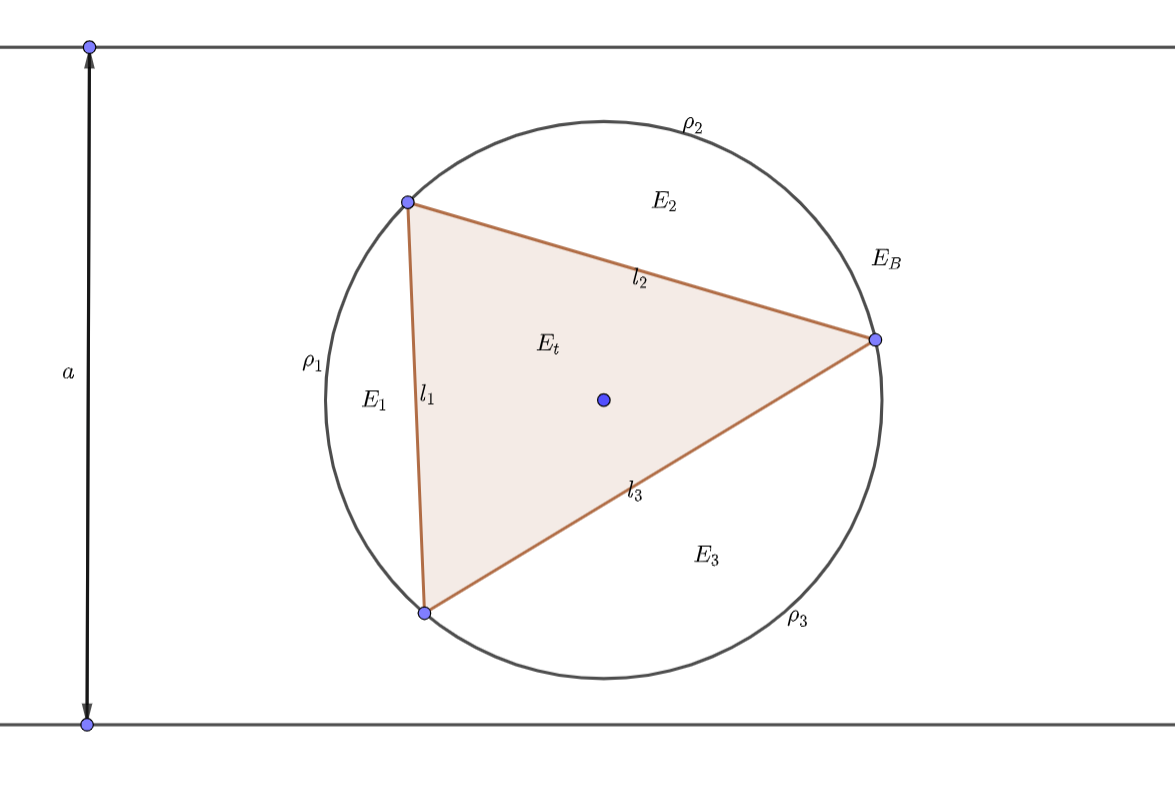
\includegraphics[width=0.8\textwidth]{figure.png}
}
\fi
\iffalse
% 表格模板
\renewcommand\arraystretch{0.8} % 设置表格高度为原来的0.8倍
\begin{table}[!htbp] % table标准
    \centering % 表格居中
    \begin{tabular}{p{1cm}<{\centering}p{1cm}<{\centering}p{3cm}<{\centering}p{5cm}<{\centering}} % 设置表格宽度
    %\begin{tabular}{cccc}
        \toprule
        $x_i$ & $f[x_1]$ & $f[x_i,x_{i+1}]$ & $f[x_i,x_{i+1},x_{i+2}]$ \\
        \midrule
        $x_0$ & $f(x_0)$ &                  &                          \\
        $x_0$ & $f(x_0)$ & $f'(x_0)$        &                          \\
        $x_0$ & $f(x_1)$ & $\frac{f(x_1)-f(x_0)}{x_1-x_0}$ & $\frac{f(x_1)-f(x_0)}{(x_1-x_0)^2}-\frac{f'(x_0)}{x_1-x_0}$\\
        \bottomrule
    \end{tabular}
\end{table}
\fi

\end{document}